Let    
    \begin{align}    
    \vec{A} = \myvec{21\\-2},
    \vec{B} = \myvec{15\\10},
    \vec{C} = \myvec{-5\\0},
    \vec{D} = \myvec{1\\-12}\label{rams/1/1/10/eq 2.0.1}
    \end{align}
    Then, 
    \begin{align}
        \vec{A} - \vec{B} *= \myvec{6 \\ -12}
    \\
    \vec{B} - \vec{C}     &= \myvec{20 \\ 10}
    \\
    \vec{C} - \vec{D}      & = \myvec{-6 \\ 12}
    \\
    \vec{D} - \vec{A}    & = \myvec{-20 \\ -10}
    \end{align}
    Since the directional vectors of $\vec{AB}$ and $\vec{CD}$
    are in the same ratio, so  $\vec{AB}$ and $\vec{CD}$ are
    parallel and also opposite to each other.
    Similarly, $\vec{BC}$ and $\vec{DA}$ are parallel and opposite.
    %
    Hence ABCD is a parallelogram.  Also, 
    \begin{align}
     (\vec{\vec{B} - \vec{A}})^\top(\vec{\vec{C} - \vec{B}}) 
        &= \myvec{-6 & 12} \myvec{-20 \\ -10}\\
        &= 0
    \end{align}
    Therefore, one of the angle is right angle and ABCD is a rectangle.
    The center
    \begin{align}
        \vec{O} &= \frac{\vec{A}+ \vec{C}}{2}\\
        &= \myvec{8 \\ -1}
    \end{align}
    This is verified in Fig. \ref{rams/1/1/10/fig:my_label}.
    \begin{figure}[htp]
        \centering
        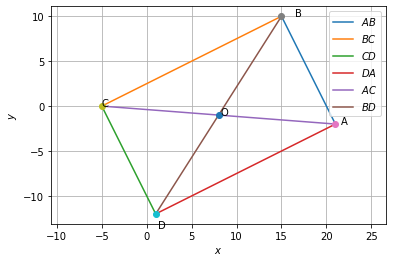
\includegraphics[width=\columnwidth]{solutions/1/1/10/Figure/AS1.png}
        \caption{plot}
        \label{rams/1/1/10/fig:my_label}
    \end{figure}